\documentclass[10pt,letterpaper]{article}
\usepackage[top=0.85in,left=1.0in,right=1.0in,footskip=0.75in]{geometry}

% Use adjustwidth environment to exceed column width (see example table in text)
\usepackage{changepage}

% Use Unicode characters when possible
\usepackage[utf8]{inputenc}

% textcomp package and marvosym package for additional characters
\usepackage{textcomp,marvosym}

% fixltx2e package for \textsubscript
\usepackage{fixltx2e}

% amsmath and amssymb packages, useful for mathematical formulas and symbols
\usepackage{amsmath,amssymb}

% cite package, to clean up citations in the main text. Do not remove.
\usepackage{cite}

% Use nameref to cite supporting information files (see Supporting Information section for more info)
\usepackage{nameref,hyperref}

\usepackage{amsthm}

% line numbers
\usepackage[right]{lineno}

% ligatures disabled
\usepackage{microtype}
\DisableLigatures[f]{encoding = *, family = * }

% rotating package for sideways tables
\usepackage{rotating}

% Remove comment for double spacing
%\usepackage{setspace} 
%\doublespacing

% Text layout
\raggedright
\setlength{\parindent}{0.5cm}
\textwidth 6.25in 
\textheight 8.75in

% Bold the 'Figure #' in the caption and separate it from the title/caption with a period
% Captions will be left justified
\usepackage[aboveskip=1pt,labelfont=bf,labelsep=period,justification=raggedright,singlelinecheck=off]{caption}

% Use the PLoS provided BiBTeX style
\bibliographystyle{plos2015}

% Remove brackets from numbering in List of References
\makeatletter
\renewcommand{\@biblabel}[1]{\quad#1.}
\makeatother

\newtheorem{theorem}{Theorem}
\newtheorem{lemma}{Lemma}
\newtheorem{definition}{Definition}

% Leave date blank
\date{}

% Header and Footer with logo
\usepackage{lastpage,fancyhdr,graphicx}
\usepackage{epstopdf}
\pagestyle{myheadings}
\pagestyle{fancy}
\fancyhf{}

\rfoot{\thepage/\pageref{LastPage}}
\renewcommand{\footrule}{\hrule height 2pt \vspace{2mm}}
\fancyheadoffset[L]{2.25in}
\fancyfootoffset[L]{2.25in}
\lfoot{\sf PLOS}

%% END MACROS SECTION
\begin{document}
\vspace*{0.35in}

\begin{flushleft}
{\Large
\textbf\newline{Descent-based joint optimization}
}
\newline
\\
Jean Feng and Noah Simon
\\

\end{flushleft}
\section*{Abstract}
Tuning regularization parameters in regression problems allows one to control model complexity and induce desired structure. The current method of searching over a $k$-dimensional grid of parameter values is computationally intractable for $k>2$. We propose tuning the penalty parameters more efficiently by treating it as a continuous optimization problem and updating the parameter values using subgradient descent. We demonstrate that this method of ``joint optimization" achieves the same performance as cross validation over a grid. Joint optimization enables us to test regularizations with many penalty parameters, through which we discover new regularization methods that attain superior accuracy. Our experiments are performed on simulated and real data.

\section{Introduction}

Consider the usual regression framework with $p$ features and a response measured on $n$ observations. Let $X$ denote the $n \times p$ design matrix and $y$ the response vector. For ill-posed or high-dimensional problems ($p \gg n$), there can often be an infinite number of solutions that minimize the loss function $L$ but have high generalization error. A common solution is to use regularization, or penalization, to select models with desirable properties, such as smoothness and sparsity.

In recent years, there has been much interest in combining regularization methods to produce models with multiple desired characteristics. Examples include the elastic net (Zou and Hastie 2003), which combines the lasso and ridge penalties, and the sparse group lasso (Simon 2007), which combines the group lasso and lasso penalties. The general form of these regression problems is:

\begin{equation} \label {eq:basic}
\hat f(\lambda_1, ..., \lambda_k) = \arg \min_f L(\boldsymbol{y}, f (\boldsymbol{X})) + \sum\limits_{i=1}^k \lambda_i J_i(f)
\end{equation}
where $L$ is the loss function, $\{J_i\}_{i=1, ..., k}$ are the penalty functions, and $\{\lambda_i\}_{i=1, ..., k}$ are the regularization parameters.

Regularization parameters control the degree of various facets of model complexity (e.g. amount of sparsity or smoothness). Often, the goal is to set the parameters to minimize the fitted model's generalization error. One usually estimates this using a training/validation approach (or cross-validation). There one fits a model on a training set $(X_T, \boldsymbol y_T)$ and measures the model's error on a validation set $(X_V, \boldsymbol y_V)$. The goal then is to choose penalty parameters that minimize the validation error, as formulated in the following optimization problem:
\begin{equation}
\begin{array}{c}
\min_{\boldsymbol{\lambda} \in \Lambda} L(\boldsymbol{y}_V, \hat f (\boldsymbol{X}_V | \boldsymbol{\lambda})) \\
\text{where } \hat f(\cdot | \boldsymbol{\lambda}) = \arg \min_f L(\boldsymbol{y}_T, f (\boldsymbol{X}_T)) + \sum\limits_{i=1}^k \lambda_i J_i(f)
\end{array}
\label{jointopt}
\end{equation}

The simplest approach to solving the problem above is brute force: one fits models over a grid of parameter values and selects the model with the lowest validation error. As long as the grid is large and fine enough, this method of ``grid search" will find a solution close to the global optimum. This approach is the current standard for choosing penalty parameters via train/validation. Unfortunately, it is computationally intractable in cases with more than two parameters. Many variants of grid search have been proposed to increase efficiency, but their runtimes are all exponential in the number of parameters.

In this paper, we propose leveraging the tools of optimization to solve \eqref{jointopt} over the penalty parameter space. We give a gradient descent algorithm for the penalty parameters (to minimize validation error). In contrast to an exhaustive ``grid search'', this ``descent-based'' optimization makes use of the smoothness of our validation-error surface. 

In simulation studies we show that our descent-based optimization produces solutions with the same validation error as those from grid search. In addition, we find that our approach is highly efficient and can solve regressions with hundreds of penalty parameters. Finally, we use this method to analyze regularization methods that were previously computationally intractable. Through this, we discover that a variant of sparse group lasso with many more penalty parameters can significantly decrease error and produce more meaningful models.

Lorbert and Ramadge (2010) presented some related work on this topic. They solved linear regression problems by updating regression coefficients and regularization parameters using cyclical coordinate gradient descent. We take a more general approach that allows us to apply joint optimization to both linear and nonlinear regressions. In particular this paper focuses on three examples that demonstrate the wide applicability of our method: elastic net, sparse group lasso, and additive partial linear models.

In Section 2, we describe descent-based optimization in detail and present an algorithm for solving it in example regressions. In Section 3, we show that our method achieves validation errors as low as those achieved by grid search. In Section 4, we explore variants of the example regression problems that have many more regularization parameters and demonstrate that solving \eqref{jointopt} is still computationally tractable. Finally, we present results on data predicting colitis status from gene expression in Section 5.

\section{Descent-based Joint Optimization}
\subsection{Definition}
Suppose that we have $n$ observations on each of which we have measured $p$ features and a response. Let $\boldsymbol{y}$ be the $n$ response vector and $\boldsymbol{X}$ be the $n \times p$ design matrix. In addition, suppose we are fitting a model $f$ by minimizing a penalized criterion of the form:
\begin{equation}
L(\boldsymbol{y}, f (\boldsymbol{X})) + \sum\limits_{i=1}^k \lambda_i J_i(f)
\end{equation}
where $L$ is the loss function and $(J_i, \lambda_i)$ is the $i$th penalty function and the corresponding penalty parameter.

Suppose we would to select penalty parameters $\boldsymbol{\lambda} = (\lambda_1, ..., \lambda_k)^T$ via a training/validation split. We partition the data into a training set $(\boldsymbol{y}_T , \boldsymbol{X}_T)$ and validation set $(\boldsymbol{y}_V, \boldsymbol{X}_V)$. We choose our penalty parameters to minimize the validation error by solving the following optimization problem:
\begin{equation}
\begin{array}{c}
\arg \min_{\boldsymbol{\lambda} \in \mathbb{R}^k} L(\boldsymbol{y}_V, \hat f(\boldsymbol{X}_V | \boldsymbol{\lambda})) \\
\text{where } \hat f(\cdot | \boldsymbol{\lambda}) = \arg \min_f L(\boldsymbol{y}_T, f (\boldsymbol{X}_T)) + \sum\limits_{i=1}^k \lambda_i J_i(f)
\end{array}
\label{jointopt2}
\end{equation}

For ease of reading, we will use $L_V(\boldsymbol{\lambda})$ to denote $L(\boldsymbol y_V, \hat f(X_V | \boldsymbol{\lambda}))$ since the validation loss is ultimately a function of the penalty parameters.

\eqref{jointopt2} is the explicit, though often unstated, criterion that training/validation methods attempt to minimize to choose penalty parameters . The current standard is to minimize this using an exhaustive grid-search. Grid-based methods solve the joint optimization problem by fitting models over a $k$-dimensional grid $G$ in the penalty parameter space --- the computational runtime of grid-based methods grows exponentially with the number of parameters. While the approach is simple and powerful for a single penalty parameter, optimizing even moderate dimensional functions (3+) via exhaustive grid search is inefficient (and becomes quickly completely intractable).  In addition \eqref{jointopt2} is generally a continuous, piecewise-smooth problem. Using an exhaustive search ignores information available from the smoothness of the surface. 

We propose leveraging the tools of smooth optimization to solve \eqref{jointopt2}. In particular we discuss iterative methods, based on walking in a descent direction until convergence to a local minimum. In the simple case where the criterion is differentiable with respect to the penalty parameters, it is straightforward to use gradient descent or some variant thereof. We show that, with some slight tweaks, gradient descent can be applied in situations where the penalty is only differentiable when restricted to directions involving an active set.

Figure \ref{fig:compare} illustrates the differences between the two approaches. Grid-based method fits a model at every grid point, even though many of these grid points are not close to the global or local minima. We can save significant computational time if we avoid those points unlikely to yield good models. By incorporating information about the shape of the local neighborhood, descent-based methods choose an intelligent descent direction and explore the space more efficiently. 

\begin{figure}
\begin{center}
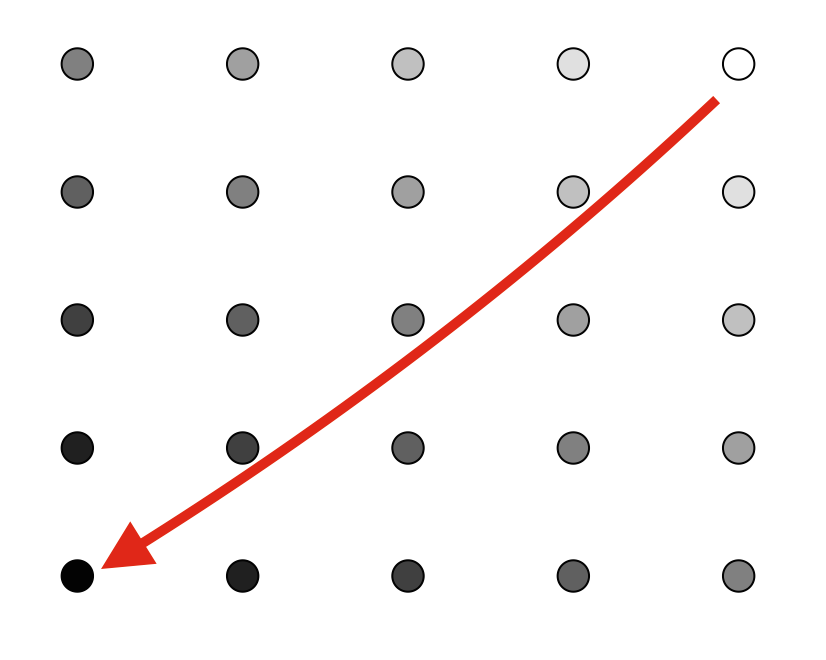
\includegraphics[height=40mm]{grid_search_vs_descent.png}
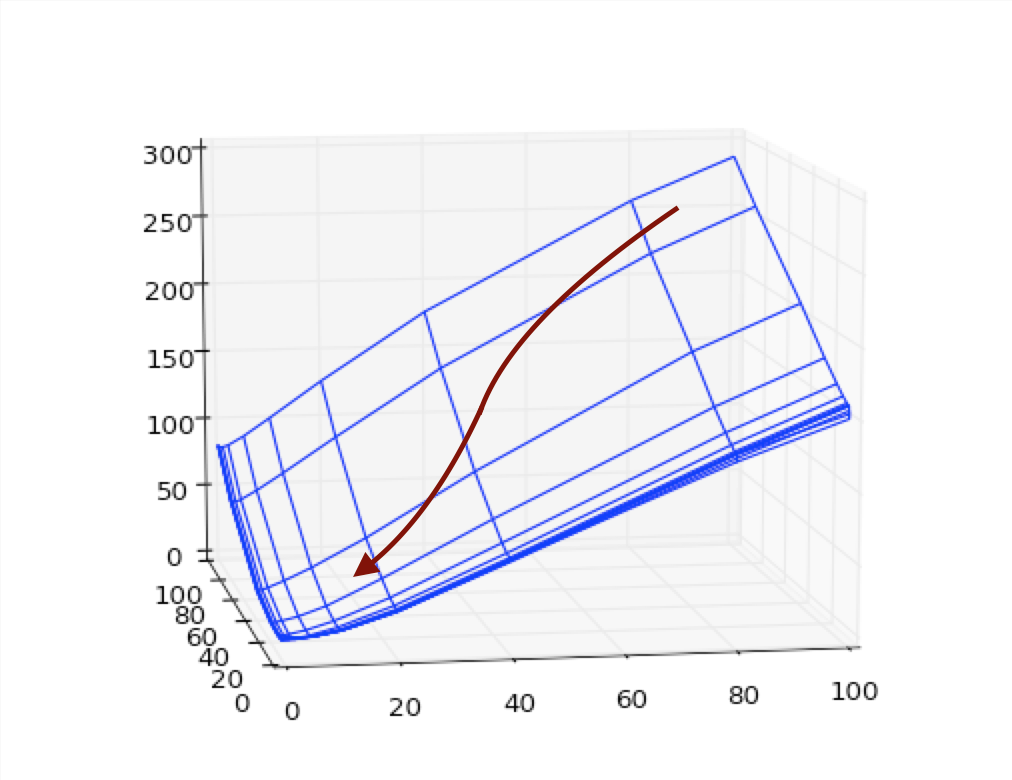
\includegraphics[height=60mm]{surface_in_regularization_parameters.png}
\end{center}
\caption{Left: darker points mean lower validation loss. Descent-based optimization descends in the most direct path towards the point producing the lowest validation loss. Right: The 3D version. We can tune regularization parameters using a grid search... or just descend opposite of the gradient.}
\label{fig:compare}
\end{figure}

Of course, the joint optimization problem is non-convex and therefore our method provides no guarantees. The major benefit of using our method is that it opens up the possibility of using regularization methods that combine multiple penalty terms.

\subsection{Gradient Descent for Joint Optimization}

In this section, we show how joint optimization problems can be solved using gradient descent. We first explain this method for the simple case where the validation loss $L_V(\boldsymbol{\lambda})$ is differentiable with respect to $\boldsymbol{\lambda}$. We then show that for cases where the validation loss is non-differentiable, we can reduce the problem and still solve it using gradient descent. Finally, we discuss variants of gradient descent that can also be used.

\subsubsection{Differentiable functions! The simple case!}

Suppose $L_V(\boldsymbol{\lambda})$ is differentiable everywhere in $\boldsymbol{\lambda}$. We can solve the joint optimization using gradient descent, as detailed in the box below:

\begin{center}
  \fbox{
    \parbox{30em}{
        Choose step size $\alpha$.\\
        Initialize $\lambda^{(0)}$.\\
        For each iteration $k$:
	\begin{equation*}
	\boldsymbol{\lambda}^{(k+1)} := \boldsymbol{\lambda}^{(k)} - \alpha \nabla{L_V}(\boldsymbol{\lambda}^{(k)})
	\end{equation*}
	% where $\boldsymbol{g}_V(\boldsymbol{\lambda}^{(k)})$ is any subgradient of $L_V$ at $\boldsymbol{\lambda}^{(k)}$.
	%where $\alpha(\lambda^{(k)})$ is the step size for the $k$th step.
    }
  }
\end{center}
The complexity in the algorithm above is hidden in the gradient term $\nabla{L_V}(\boldsymbol{\lambda})$. By the chain rule, the gradient requires calculating the gradient of the minimizer of penalized regression $\hat f$:
\begin{equation}
\nabla_\lambda{L_V}(\boldsymbol{\lambda}) = \frac{\partial}{\partial \hat f}L_V(\hat f(\boldsymbol{\lambda}))^T \frac{\partial}{\partial \lambda} \hat f(\boldsymbol{\lambda})
\label{chainrule}
\end{equation}

If there is a closed-form solution for $\hat f(\cdot | \lambda)$, this calculation is straightforward. Ridge regression is an example of this case.

However, there is usually no closed-form solution. Instead, we rely on the KKT conditions for an implicit equation of the minimizer of the penalized regression. The stationarity condition states that, at optimality, the gradient of the penalized criterion with respect to $\hat f$ is zero:
\begin{equation}
0 = \nabla_{\hat f} \bigg(L(\boldsymbol y_T, \hat f (X_T)) + \sum\limits_{i=1}^k \lambda_i J_i(\hat f) \bigg)
\label{eq:kktgradient}
\end{equation}

We then perform implicit differentiation of the equation above with respect to $\boldsymbol{\lambda}$ to get the gradient $\frac{\partial \hat f}{\partial \boldsymbol{\lambda}}$. This can then be plugged into equation \ref{chainrule} to get the gradient $\nabla{L_V}(\boldsymbol{\lambda}^{(k)})$ to perform gradient descent.

Note that the gradient $\frac{\partial \hat f}{\partial \boldsymbol{\lambda}}$ is often in terms of $\hat f$, which means that each gradient step requires solving the ``inner" optimization problem. While this may seem costly, using warm starts significantly reduces the number of iterations needed to solve the inner problem.

\subsubsection{Differentiable almost everywhere! Complicated!}

Now, consider the case where the loss function or the penalty functions are not differentiable everywhere. Under certain assumptions, we can perform a modified gradient descent, which involves restricting the problem to an active set. That is, given the model parameters $\hat f = \arg \min_f L(f)$, we define the active set at $\hat f$ as the model parameters $\hat f_i$ where the $L(\hat f)$ is twice continuously differentiable with respect to $f_i$. We use $\dot f$ to indicate the active set of $\hat f$.

If some regularity conditions are satisfied and the elements not in the active set are locally constant almost everywhere, we can perform our modified gradient descent. At each iteration, the optimization problem is restricted to the active set:

\begin{equation}
\begin{array}{c}
\arg \min_{\boldsymbol{\lambda} \in \mathbb{R}^k} L(\boldsymbol{y}_V, \dot f(\dot{\boldsymbol{X}}_V | \boldsymbol{\lambda})) \\
\text{where } \dot f(\cdot | \boldsymbol{\lambda}) = \arg \min_f L(\boldsymbol{y}_T, f (\dot{\boldsymbol{X}}_T)) + \sum\limits_{i=1}^k \lambda_i J_i(f)
\end{array}
\label{restrictedjointopt}
\end{equation}

and the descent direction is calculated very similar to before:

\begin{equation}
\nabla_\lambda L_V(\boldsymbol{\lambda}) = \frac{\partial}{\partial \dot f} L_V(\dot f(\boldsymbol{\lambda}))^T \frac{\partial}{\partial \boldsymbol{\lambda}} \dot f(\boldsymbol{\lambda})
\end{equation}

When restricting the joint optimization problem to the active set, we may need to modify the design matrix, which is why the design matrices for the training and validation set are now denoted as $\dot{\boldsymbol{X}}_T$ and $\dot{\boldsymbol{X}}_V$. For example, in the examples below, the design matrices restricted to the active set are just the subset of the columns that correspond to the active set.

This modified gradient descent is based on the following theorem, which follows directly from Lemma \ref{differentiablethrm} and \ref{activesetthrm} in the appendix.

\begin{theorem}
For the optimization problem in (\ref{jointopt2}), suppose that $L(\hat f(\boldsymbol{\lambda}))$ and
$\sum\limits_{i=1}^k \lambda_i J_i(f)$ are twice continuously differentiable almost everywhere with respect to $f$ and that the hessian of
\begin{equation}
L(\boldsymbol{y}_T, f (\boldsymbol{X}_T)) + \sum\limits_{i=1}^k \lambda_i J_i(f)
\end{equation}
with respect to $f$ is nonsingular almost everywhere. In addition, suppose that the non-active set of $\hat f(\lambda)$ is locally constant almost everywhere. Then the objective function $L_V(\boldsymbol{\lambda})$ is continuously differentiable almost everywhere with respect to $\lambda$.
\label{thethrm}
\end{theorem}

Many penalized regressions satisfy the assumptions, such as the example regressions in this paper. One case that doesn't hold is lasso regression for high-dimensional datasets (the nonsingularity requirement is violated), but adding a ridge penalty with a tiny coefficient will be sufficient.

\subsubsection{Variants of Gradient Descent}

Joint optimization problems can also be solved using variants of gradient descent. Instead of a constant step size $\alpha$, one can use decreasing or adaptive step sizes $\alpha(\lambda^{(k)})$. In our simulation studies, we implement both regular gradient descent and Nesterov's gradient descent with adaptive restarts. Nesterov's gradient descent is an accelerated method in which the step size depends on previous steps, and the momentum grows from one iteration to the next. Restarting refers to resetting the momentum back to zero. In our implementation of Nesterov's gradient descent with adaptive restarts, we restart whenever the criterion increases in value. For more details, refer to the analysis by O'Donaghue and Candes.

\subsection{Joint optimization for example regressions}

In this subsection, we present example joint optimization problems and derivations for the gradient. We begin with the simple example of ridge regression, followed by the more complex examples elastic net, sparse group lasso, and additive partial linear models.

\subsubsection{Ridge Regression}

The joint optimization problem for ridge regression is:
\begin{equation}
\begin{array}{c}
\min_{\lambda\in \mathbb{R}} \frac{1}{2} \lvert\lvert \boldsymbol{y}_V - \boldsymbol{X}_V \hat{\boldsymbol{\beta}} (\lambda) \rvert\rvert ^2 \\
\text{  where  } \hat{\boldsymbol{\beta}} (\lambda) = \arg \min_{\boldsymbol{\beta}} \frac{1}{2} \lvert\lvert \boldsymbol{y}_T - \boldsymbol{X}_T \boldsymbol{\beta} \rvert\rvert ^2 + \lambda \lvert\lvert \boldsymbol{\beta} \rvert\rvert_2^2
\end{array}
\end{equation}

Calculating the gradient is straightforward since there is a closed-form solution for $\hat{\boldsymbol{\beta}}(\lambda)$:
\begin{equation}
\hat{\boldsymbol{\beta}} (\lambda) = (\boldsymbol{X}_T^T\boldsymbol{X}_T + \lambda \boldsymbol{I})^{-1}\boldsymbol{X}_T^T\boldsymbol{y}_T
\end{equation}

Differentiating the above equation with respect to $\lambda$ and then using the chain rule gives us the gradient:

\begin{equation}
\begin{array} {lcl}
\nabla_\lambda L_V(\lambda)
&=& (\boldsymbol{X}_V(\boldsymbol{X}_T^T \boldsymbol{X}_T + \lambda \boldsymbol{I})^{-1}
\hat{\boldsymbol{\beta}})^T(\boldsymbol{y}_V - \boldsymbol{X}_V \hat{\boldsymbol{\beta}}(\lambda))
\end{array}
\end{equation}

\subsubsection{Elastic Net}

The elastic net combines the $\ell_1$ and $\ell_2$ penalties to address the limitations of lasso and ridge regression. Joint optimization finds the optimal regularization parameters $\boldsymbol{\lambda} = (\lambda_1, \lambda_2)^T$ corresponding to each of these penalties:

\begin{equation}
\begin{array}{c}
\min_{\boldsymbol{\lambda} \in \mathbb{R}^2} \frac{1}{2} \lvert\lvert \boldsymbol{y}_V - \boldsymbol{X}_V \hat{\boldsymbol{\beta}} (\lambda) \rvert\rvert ^2 \\
\text{ where }
\hat{\boldsymbol{\beta}} (\boldsymbol{\lambda}) = \arg \min_{\boldsymbol{\beta}} \frac{1}{2} \lvert\lvert \boldsymbol{y}_T - \boldsymbol{X}_T \boldsymbol{\beta} \rvert\rvert ^2
+ \lambda_1 \lvert\lvert \boldsymbol{\beta} \rvert \rvert_1
+ \frac{1}{2}\lambda_2 \lvert\lvert \boldsymbol{\beta} \rvert \rvert_2^2
\end{array}
\end{equation}

By the KKT conditions, we have that:
\begin{equation}
0 \in -\boldsymbol{X}_T^T(\boldsymbol{y}_T
- \boldsymbol{X}_T \hat{\boldsymbol{\beta}} (\boldsymbol{\lambda}) )
+ \lambda_1 s(\hat{\boldsymbol{\beta}} (\boldsymbol{\lambda}))
+ \lambda_2 \hat{\boldsymbol{\beta}} (\boldsymbol{\lambda})
\end{equation}
where $s$ is the subgradient of the lasso penalty and is defined by

\begin{equation}
s(\beta_i) = \begin{cases}
  sign(\beta_i) & \text{if } \beta_i \ne 0, \\
  [-1, 1] & \text{otherwise}
\end{cases}
\end{equation}

We reduce the problem to just a gradient equation by restricting the features to the active set where $\boldsymbol \beta_i \ne 0$. Let $\dot{\boldsymbol{\beta}}(\boldsymbol \lambda)$ be the active regression coefficients and $\dot{\boldsymbol{X}}_T$ and $\dot{\boldsymbol{X}}_V$ be the reduced design matrices. We get the following equation:

\begin{equation}
-\dot{\boldsymbol{X}}_T^T(\boldsymbol y_T - \dot{\boldsymbol{X}}_T \dot{\boldsymbol{\beta}} (\boldsymbol{\lambda}) )
+ \lambda_1 sign(\dot{\boldsymbol{\beta}} (\boldsymbol{\lambda}))
+ \lambda_2 \dot{\boldsymbol{\beta}}(\boldsymbol{\lambda}) = 0
\end{equation}

Performing implicit differentiation gives us the gradient:

\begin{equation}
\nabla_\lambda L_V(\boldsymbol{\lambda}) =
\begin{bmatrix}
(\dot{\boldsymbol{X}}_V^T(\dot{\boldsymbol{X}}_T^T \dot{\boldsymbol{X}}_T + \lambda_2 \boldsymbol{I})^{-1}
sign(\dot{\boldsymbol{\beta}} (\boldsymbol{\lambda})))^T
(\boldsymbol y_V - \dot{\boldsymbol{X}}_V \dot{\boldsymbol{\beta}} (\boldsymbol{\lambda}))\\
(\dot{\boldsymbol{X}}_V^T(\dot{\boldsymbol{X}}_T^T \dot{\boldsymbol{X}}_T + \lambda_2 \boldsymbol{I})^{-1} \dot{\boldsymbol{\beta}} (\boldsymbol{\lambda}))^T
(\boldsymbol y_V - \dot{\boldsymbol{X}}_V \dot{\boldsymbol{\beta}} (\boldsymbol{\lambda}))
\end{bmatrix}
\end{equation}

\subsubsection{Sparse Group Lasso}

Sparse group lasso, a variant of the classical lasso regression, is intended for modeling problems with grouped covariates believed to have sparse effects on a group and a within-group level. Given $m$ covariate groups, let the predictors $\boldsymbol{X}$ and coefficient vector $\boldsymbol \beta$ be split into submatrices $\boldsymbol{X}^{(k)}$ and vectors $\boldsymbol \beta^{(k)}$ for each covariate group $k = 1, ... , m$. Sparse group lasso enforces group-level sparsity and within-group sparsity using the penalties $\sum_{k=1}^m \lvert\lvert \boldsymbol\beta^{(k)} \rvert \rvert_2$ and $||\boldsymbol\beta ||_1$. The joint optimization problem to get the optimal regularization parameters $\boldsymbol{\lambda} = (\lambda_1, \lambda_2)^T$ is:

\begin{equation}
\begin{array}{c}
\min_{\boldsymbol{\lambda} \in \mathbb{R}^2} \frac{1}{2n} \bigl\lvert\bigl\lvert \boldsymbol{y}_V - X_V \hat{\boldsymbol{\beta}}(\boldsymbol{\lambda}) \bigl\rvert\bigl\rvert^2_2 \\
\text{ where }
\hat{\boldsymbol{\beta}}(\boldsymbol{\lambda}) = \arg\min_{\boldsymbol{\beta}} \frac{1}{2n} \bigl\lvert\bigl\lvert \boldsymbol{y}_T - \boldsymbol{X}_T \boldsymbol{\beta} \bigl\rvert\bigl\rvert^2_2
+ \lambda_1 \sum_{k=1}^m \lvert\lvert \boldsymbol\beta^{(k)} \rvert \rvert_2
+ \lambda_2 \lvert\lvert \boldsymbol\beta \rvert \rvert_1
\end{array}
\end{equation}

The KKT conditions state that
\begin{equation}
0 \in -\boldsymbol{X}_T^T(\boldsymbol{y}_T - \boldsymbol{X}_T \hat{\boldsymbol{\beta}}(\boldsymbol{\lambda}))
+ \lambda_1 \sum\limits_{l=1}^m t(\hat{\boldsymbol{\beta}}^{(k)}(\boldsymbol{\lambda}))
+ \lambda_2 s(\hat{\boldsymbol{\beta}}^{(k)}(\boldsymbol{\lambda}))
\end{equation}
where $s$ was defined previously. The subgradient of the group lasso penalty $t$ is defined as

\begin{equation}
t(\boldsymbol{\beta}^{(k)}(\boldsymbol{\lambda})) = \begin{cases}
  \frac{ \hat{\boldsymbol{\beta}}^{(k)}(\boldsymbol{\lambda})}{||\hat{\boldsymbol{\beta}}^{(k)}(\boldsymbol{\lambda}) ||_2} & \text{if } \boldsymbol\beta^{(k)} \ne \boldsymbol{0}, \\
\{t : ||t||_2 \le 1\} & \text{otherwise}
\end{cases}
\end{equation}

We reduce the problem by restricting to just the active set of features, which are those with nonzero coefficients $\boldsymbol{\beta}^{(k)}_i$. The reduced stationarity equation, in terms of the active regression coefficients $\dot{\boldsymbol{\beta}} (\lambda)$ and reduced design matrices $\dot{\boldsymbol{X}}_T$ and $\dot{\boldsymbol{X}}_V$, is

\begin{equation}
\nabla_\lambda L_V(\boldsymbol{\lambda}) =
\begin{bmatrix}
\frac{1}{n}
\Bigg (
\dot{\boldsymbol{X}}_V
(\frac{1}{n} \dot{\boldsymbol{X}}_T^T \dot{\boldsymbol{X}}_T - \lambda_1 \boldsymbol{M}_1 + \lambda_1 \boldsymbol{M}_2)^{-1}
t(\dot{\boldsymbol{\beta}}(\boldsymbol{\lambda}))
\Bigg )^T
(\boldsymbol{y}_V - \dot{\boldsymbol{X}}_V \dot{\boldsymbol{\beta}})
 \\
\frac{1}{n}
\Bigg (\dot{\boldsymbol{X}}_V
(\frac{1}{n} \dot{\boldsymbol{X}}_T^T \dot{\boldsymbol{X}}_T - \lambda_1 \boldsymbol{M}_1 + \lambda_1 \boldsymbol{M}_2)^{-1}
s(\dot{\boldsymbol{\beta}}(\boldsymbol{\lambda}))
\Bigg )^T
(\boldsymbol{y}_V - \dot{\boldsymbol{X}}_V \dot{\boldsymbol{\beta}})
\\ 
\end{bmatrix}
\end{equation}

where $\boldsymbol{M}_1$ is the block diagonal matrix with  components 
$
|| \dot{\boldsymbol{\beta}}^{(k)}(\boldsymbol{\lambda})||_2^{-3} \dot{\boldsymbol{\beta}}^{(k)}(\boldsymbol{\lambda}) \dot{\boldsymbol{\beta}}^{(k)}(\boldsymbol{\lambda})^T
$ and $\boldsymbol{M}_2$ is the block diagonal matrix with components
$||\dot{\boldsymbol{\beta}}^{(k)}(\boldsymbol{\lambda})||_2^{-1} \boldsymbol{I}$
for $k = 1, ..., m$ 
from top left to bottom right.

\subsubsection{Additive Partial Linear Models}

Additive partial linear models (APLMs), a semi-parametric regression model, is used when the response is believed to depend on some of the predictors linearly and the other predictors nonlinearly. More specifically, given the predictors $\boldsymbol x \in \mathbb{R}^{n}$ and $z \in \mathbb{R}$, the predicted response $y$ is $\boldsymbol x^T\boldsymbol \beta + g(z)$, where $\boldsymbol \beta$ is the regression coefficients and $g$ is some nonlinear univariate function.

For this example, the APLM uses a lasso penalty for the linear component and an $\ell_2$ trend-filtering penalty for the nonlinear component. Let the data set have linear predictors $\boldsymbol{X} \in \mathbb{R}^{n \times p}$ and nonlinear predictors $\boldsymbol{z} \in \mathbb{R}^n$. We assume that the observations are ordered by increasing $z_i$. The training set $\boldsymbol{X}_T$ is randomly chosen from the data and can be obtained using matrix multiplication $ \boldsymbol{X}_T = \boldsymbol{M}_T \boldsymbol{X}$ for some matrix $\boldsymbol{M}_T$. The validation set $\boldsymbol{X}_V$, composed of the remaining observations, are obtained using a similarly defined matrix $\boldsymbol{M}_V$.
The joint optimization problem to obtain the optimal penalty parameters $\boldsymbol\lambda = (\lambda_1, \lambda_2)^T$ is as follows:
\begin{equation}
\begin{array}{c}
\min_{\boldsymbol\lambda \in \mathbb{R}^2} \frac{1}{2}
\bigl\lvert\bigl\lvert
\boldsymbol{y}_V
- \boldsymbol{X}_V\hat{\boldsymbol{\beta}}(\boldsymbol{\lambda})
- \boldsymbol{M}_V \hat{\boldsymbol{\theta}}(\boldsymbol{\lambda})
\bigl\rvert\bigl\rvert^2_2 \\
\text{ where } \hat{\boldsymbol{\beta}}(\boldsymbol{\lambda}),
\hat{\boldsymbol{\theta}}(\boldsymbol{\lambda}) =
\arg\min_{\boldsymbol{\beta}, \boldsymbol{\theta}}
\frac{1}{2} \bigl\lvert\bigl\lvert
\boldsymbol{y}_T
- \boldsymbol{X}_T\boldsymbol{\beta}
- \boldsymbol{M}_T \boldsymbol{\theta} \bigl\rvert\bigl\rvert^2_2
+ \lambda_1 \lvert\lvert \boldsymbol{\beta}
\rvert \rvert_1
+ \frac{1}{2} \lambda_2 \lvert\lvert \boldsymbol{D} \boldsymbol{\theta} \rvert \rvert_2^2
\end{array}
\end{equation}

$\boldsymbol{D}$ is the second-order difference matrix for $\boldsymbol{z}$:
\begin{equation}
\boldsymbol{D} = \boldsymbol{D}^{(1)} \cdot
\text{diag} \big ( \frac{1}{z_{2} - z_1}, \frac{1}{z_{3} - z_2}, ... , \frac{1}{z_{n} - z_{n-1}}, 0 \big )
\cdot \boldsymbol{D}^{(1)}
\end{equation}
where
\begin{equation}
\boldsymbol{D}^{(1)} = 
\begin{bmatrix}
-1 & 1 & 0 & ... & 0 & 0 \\
0 & -1 & 1 & ... & 0 & 0 \\
\vdots \\
0 & 0 & 0 & ... & -1 & 1 \\
0 &0 & 0 &  0  &  0 & 0
\end{bmatrix}
\in
\mathbb{R}^{n\times n}
\end{equation}

The KKT conditions state that:
\begin{equation}
\begin{array}{lcl}
\boldsymbol{0} &\in&
-\boldsymbol{X}_T^T(\boldsymbol{y}_T -
\boldsymbol{X}_T \hat{\boldsymbol{\beta}}(\boldsymbol{\lambda}) - \boldsymbol{M}_T \hat{\boldsymbol{\theta}}(\boldsymbol{\lambda}))
+ \lambda_1 s(\hat{\boldsymbol{\beta}}(\boldsymbol{\lambda})) \\
\boldsymbol{0} &=&
-\boldsymbol{M}_T^T(\boldsymbol{y}_T
- \boldsymbol{X}_T \hat{\boldsymbol{\beta}}(\boldsymbol{\lambda})
- \boldsymbol{M}_T \boldsymbol{\theta}(\boldsymbol{\lambda}))
+ \lambda_2 \boldsymbol{D} \hat{\boldsymbol{\theta}}(\boldsymbol{\lambda})
\end{array}
\end{equation}

We reduce first equation to an implicit equation involving gradients. We restrict the problem to involve just the active set of features that correspond to nonzero $\beta_i$. Let the active regression coefficients be $\dot{\boldsymbol{\beta}}(\boldsymbol{\lambda})$ and reduced design matrices be $\dot{\boldsymbol{X}}_T$ and $\dot{\boldsymbol{X}}_V$. The subgradient condition is therefore reduced to the following equation:

\begin{equation}
\begin{array}{lcl}
\boldsymbol{0} &=&
-\dot{\boldsymbol{X}}_T^T(\boldsymbol{y}_T
- \dot{\boldsymbol{X}}_T \dot{\boldsymbol{\beta}}(\boldsymbol{\lambda})
- \boldsymbol{M}_T \hat{\boldsymbol{\theta}}(\boldsymbol{\lambda}))
+ \lambda_1 s(\dot{\boldsymbol{\beta}}(\boldsymbol{\lambda}))
\end{array}
\end{equation}

By the chain rule, the gradient is:
\begin{equation}
\nabla_\lambda L_V(\boldsymbol{\lambda})_i =
- \bigg(
\dot{\boldsymbol{X}}_V \frac{\partial \dot{\boldsymbol{\beta}}(\boldsymbol{\lambda})}{\partial \lambda_i}
+ \boldsymbol{M}_V \frac{\partial \hat{\boldsymbol{\theta}}(\boldsymbol{\lambda})}{\partial \lambda_i}
\bigg )^T
\bigg (
\boldsymbol{y}_V
- \dot{\boldsymbol{X}}_V \dot{\boldsymbol{\beta}}(\boldsymbol{\lambda})
- \boldsymbol{M}_V\hat{\boldsymbol{\theta}}(\boldsymbol{\lambda})
\bigg )
\text{ for } i = 1,2 
\end{equation}

The partial derivatives are obtained from implicit differentiation of the reduced KKT conditions.
\begin{equation}
\begin{array}{lcl}
\frac{\partial}{\partial \lambda_1} \dot{\boldsymbol{\beta}}(\boldsymbol{\lambda})  &=&
-\bigg(\dot{\boldsymbol{X}}_T^T \dot{\boldsymbol{X}}_T
- \dot{\boldsymbol{X}}_T^T \boldsymbol{M}_T(\boldsymbol{M}_T^T \boldsymbol{M}_T
+ \lambda_2 \boldsymbol{D}^T\boldsymbol{D})^{-1} \boldsymbol{M}_T^T \dot{\boldsymbol{X}}_T \bigg)^{-1} 
s( \dot{\boldsymbol{\beta}}(\boldsymbol{\lambda})) \\
\frac{\partial }{\partial \lambda_1} \hat{\boldsymbol{\theta}}(\boldsymbol{\lambda}) &=&
-\bigg(\boldsymbol{M}_T^T \boldsymbol{M}_T
+ \lambda_2 \boldsymbol{D}^T \boldsymbol{D}\bigg)^{-1}
\boldsymbol{M}_T^T \dot{\boldsymbol{X}}_T \frac{\partial}{\partial \lambda_1} \dot{\boldsymbol{\beta}}(\boldsymbol{\lambda})
\\
\frac{\partial}{\partial \lambda_2}  \hat{\boldsymbol{\theta}}(\boldsymbol{\lambda}) &=&
-\bigg(\boldsymbol{M}_T^T \boldsymbol{M}_T
- \boldsymbol{M}_T^T \dot{\boldsymbol{X}}_T (\dot{\boldsymbol{X}}_T^T\dot{\boldsymbol{X}}_T)^{-1} \dot{\boldsymbol{X}}_T^T \boldsymbol{M}_T + \lambda_2 \boldsymbol{D}^T\boldsymbol{D} \bigg)
\boldsymbol{D}^T\boldsymbol{D} \hat{\boldsymbol{\theta}}(\boldsymbol{\lambda})
\\
\frac{\partial}{\partial \lambda_2} \dot{\boldsymbol{\beta}}(\boldsymbol{\lambda}) &=&
- \bigg( \dot{\boldsymbol{X}}_T^T\dot{\boldsymbol{X}}_T\bigg)^{-1}
\dot{\boldsymbol{X}}_T^T \boldsymbol{M}_T
\frac{\partial}{\partial \lambda_2}  \hat{\boldsymbol{\theta}}(\boldsymbol{\lambda})\\
\end{array}
\end{equation}


\section{Results: validation error minimization}

We first address the question of whether or not joint optimization can achieve validation loss values as low as grid search. The key metrics in this comparison are, obviously, the average validation loss values for the fitted models and runtime.

We ran our experiments for the example regressions elastic net, sparse group lasso, and APLMs on simulated data. Joint optimization was implemented using gradient descent and Nesterov's gradient descent with adaptive restarts to understand how different implementations affects results. We first delineate the simulation settings and follow with a discussion of the results.

\subsection{Elastic net}
We generated 30 datasets with 80 training and 20 validation observations each and 250 predictors. For the coefficient vector $\beta$, the first 15 values were ones and the rest were zeroes. The pairwise correlation between $x_i$ and $x_j$ was set to be $corr(i,j) = 0.5^{|i-j|}$. The response vector $y$ was constructed as
\begin{equation}
y = X\beta + \sigma \epsilon
\end{equation}
where $\epsilon \sim N(0, 1)$. $\sigma$ was chosen such that the signal to noise ratio is 2.

Joint optimization was initialized at two points (0.01, 0.01) and (10, 10). Grid search was implemented over a $10 \times 10$ grid, starting from 1e-5 to four times the largest eigenvalue of $X_T^T X_T$.

\subsection{Sparse group lasso}

We generated 30 datasets of 60 training and 15 validation observations with 1500 covariates. The predictors $X$ were generated iid gaussian. The response $y$ was constructed as
\begin{equation}
y = \sum\limits_{l=1}^3 X^{(k)} \beta^{(k)} + \sigma \epsilon
\end{equation}
where $\epsilon \sim N(0, 1)$, $\beta^{(k)} = (1, 2, 3, 4, 5, 0, ..., 0)$ for $l = 1, 2, 3$. $\sigma$ was chosen such that the signal to noise ratio was 2. The number of groups $m$ in the criterion was set to 150.

Joint optimization was initialized at three points, where all regularization parameters were set to 0.01, 1, and 100. Grid search used a $10 \times 10$ grid, starting from 1e-5 to $\max(\{||X^{(k)T}y ||_2\}_{l=1,..., m})$.

\subsection{Additive partial linear models}

We generated 30 datasets with 100 training and 25 validation observations and 21 predictors. The first 20 predictors was the input for the linear function and the last predictor was the input to the nonlinear function. Predictors for the linear function were generated such that the first two groups of three features were highly correlated and the rest of the features were generated iid Gaussian.
\begin{equation}
\begin{array}{c}
x_i = Z_1 + \epsilon_i \text{ for } i=1, 2, 3 \\
x_i = Z_2 + \epsilon_i \text{ for } i= 4, 5, 6 \\
x_i \sim N(0,1) \text{ for } i = 7, ..., 20
\end{array}
\end{equation}
where $Z_1 \sim N(0,1)$, $Z_2 \sim N(0,1)$, and $\epsilon_i \sim N(0, \frac{1}{16})$. The predictors for the nonlinear component $z$ were randomly drawn from a uniform distribution from 0 to 1. The response $y$ was constructed as
\begin{equation}
y = X\beta + \kappa g(z) + \sigma \epsilon
\end{equation}
The constants $\kappa$ and $\sigma$ were chosen such that the linear to nonlinear ratio $\frac{||X\beta||_2}{||g(Z)||_2}$ was 2 and the signal to noise ratio was 2, respectively. We set $\beta = (1, 1, 1, 1, 1, 1, 0, ..., 0)$ and $g(z) =(2-z)\sin(20z^4)$.

Joint optimization was initialized at the four points $\lambda_1 = \lambda_2 = 10^i$ for $i=-2, ..., 1$. Grid search was performed over a $10 \times 10$ grid, with values ranging from $1e-6$ to $10$.


\begin{table} 
\begin{center}

\begin{tabular}{| l | l | l | l | }
\hline
\multicolumn{3}{|c|}{Elastic Net}\\
\hline
 & Validation Error & Runtime (sec) \\
\hline
Grid search & 0.34 (0.003) & 10.74\\
\hline
Gradient Descent & 0.34 (0.003) & 4.43 \\
\hline
Nesterov's Gradient Descent & 0.34 (0.003) & 2.28 \\
\hline
\end{tabular}


\begin{tabular}{| l | l | l | l | l | }
\hline
\multicolumn{3}{|c|}{Sparse Group Lasso}\\
\hline
 & Validation Error & Runtime (sec) \\
\hline
Grid search & 1.36 (0.09) & 161.29 \\
\hline
Gradient Descent  & 1.36 (0.09) & 71.34 \\
\hline
Nesterov's Gradient Descent  & 1.36 (0.10) & 67.10 \\
\hline
\end{tabular}

\begin{tabular}{| l | l | l | l | l | }
\hline
\multicolumn{3}{|c|}{APLM}\\
\hline
 & Validation Error & Runtime (sec) \\
\hline
Grid search  & 1.31 (0.05) & 27.82 \\
\hline
Gradient Descent  & 1.31 (0.05) & 16.04 \\
\hline
Nesterov's Gradient Descent  & 1.31 (0.05) & 12.09 \\
\hline
\end{tabular}

\end{center}
\caption {Validation Error comparisons}
\label{table:validation}
\end{table}


\begin{figure} 
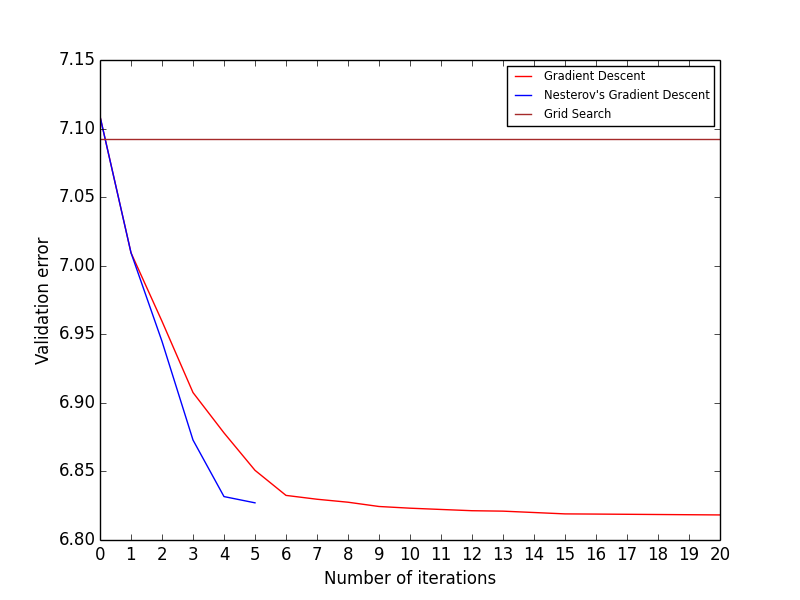
\includegraphics[width=70mm]{elasticnet_costpath_80_250_15.png}
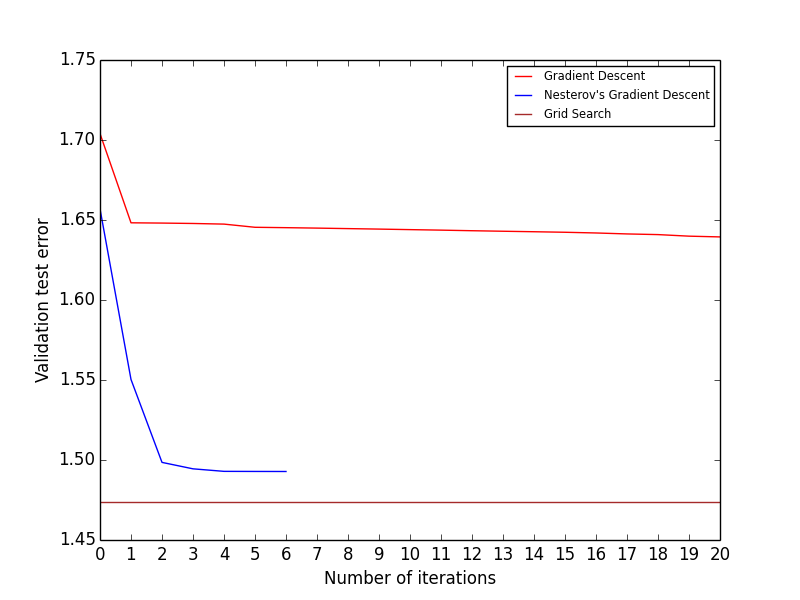
\includegraphics[width=70mm]{grouped_lasso_60_1500_3_150.png}
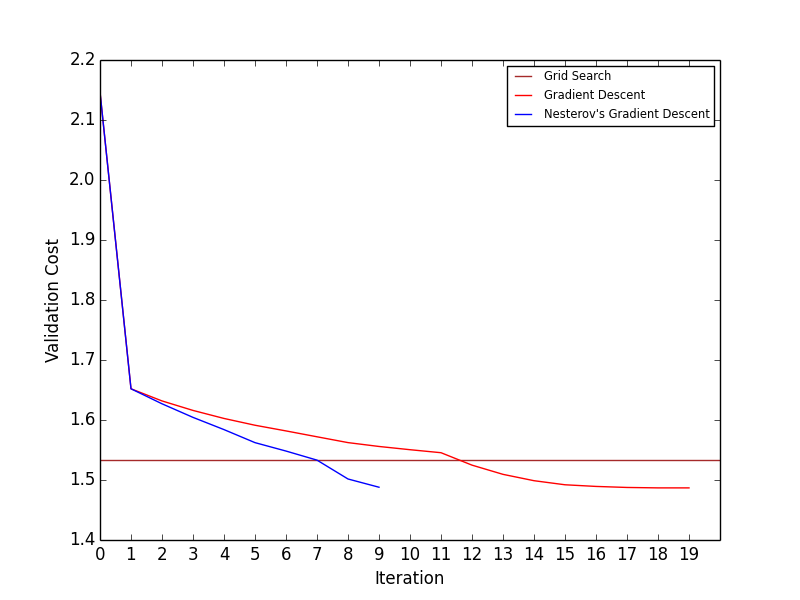
\includegraphics[width=70mm]{smooth_linear_simple_cost_path_1_100_20_6.png}
\caption{Validation error progression: Top Left - Elastic Net, Top Right - Grouped Lasso, Bottom Left - APLM}
\label{figure:costpath}
\end{figure}

\subsection{Discussion of results}

Joint optimization and grid search had the same performance in the experiments for all three example regressions. As shown in Table \ref{table:validation} ,
the only difference between grid search and joint optimization is the runtime. As hypothesized, subgradient descent and Nesterov's subgradient descent were much faster than grid search. For all the regression examples, subgradient descent was over 40\% faster and Nesterov's subgradient descent was over 50\% faster.

In addition, Figure \ref{figure:costpath} are example plots of how validation error decreases as joint optimization tunes the regularization parameters. The lowest validation error achieved by grid search is plotted as a horizontal line as reference. In general, Nesterov's subgradient descent requires fewer iterations to find the local minima.

(Do we need to be concerned that we have only shown that grid search and joint optimization produces similar results for criterions with 2 regularization parameters)

\section{Results: regularizations with more than two penalties}

This section shows that joint optimization can effectively and efficiently solve regressions with over two regularization parameters.

We created more complex criterions for the experiments by generalizing the two of the previously mentioned regression examples. For the sparse group lasso, we increased the number of regularization parameters to one plus the number of covariate groups. For the APLM example, we increased the number of regularization parameters to three. For each example, we fitted models using joint optimization and compared against models produced by grid search applied to the original two-penalty problem.

Joint optimization formulations and gradient derivations of these criterions with  are included in the Appendix.

\subsection{Unpooled sparse group lasso}

In sparse group lasso, because all $m$ covariate groups share the same two regularization parameters, the thresholds for setting coefficients and coefficient groups to zero are also shared (CITE). Here, we propose a variant of sparse group lasso such that each covariate group has an individual regularization parameter. This generalization allows for different thresholds for each coefficient and coefficient group, which is a more accurate assumption when modeling covariate groups with very different distributions. The new penalty, which we call "unpooled" sparse group lasso, replaces the original $\lambda_1$ parameter with a set of parameters $\{\lambda_1^{(k)}\}_{l=1,...,m}$:

\begin{equation}
\sum_{l=1}^m \lambda_1^{(k)} \lvert\lvert \beta^{(k)} \rvert \rvert_2
+ \lambda_2 \lvert\lvert \beta \rvert \rvert_1
\end{equation}

To compare the performance of regularization to the original sparse group lasso, we simulate data using the same settings as before. The regularization parameters for unpooled sparse group lasso were initialized at a lower set of values 1e-4, 1e-3, and 1e-2 to compensate for the fact that there are now $m + 1$ regularization parameters. In total, we performed three experiments, varying the number of covariates and the number of covariate groups $m$. 

We measured three metrics for model performance: test error, $\beta$ error, which is defined as $\lvert \lvert \beta - \hat \beta \rvert \rvert_2 ^2$, and the number of nonzero coefficients correctly identified out of the total number of nonzero coefficients in the fitted model.

As seen in Table \ref{table:unpooled}, unpooled sparse group lasso performs better by all metrics in all the experiments. The runtime for joint optimization, even when there are 150 regularization parameters, is still faster than running grid search over the two regularization parameters in sparse group lasso.

\begin{table}
\begin{center}
\begin{tabular}{| l | l | l | l | l | }
\hline
\multicolumn{5}{|c|}{n=60, p=300, g=3, m=30}\\
\hline
 & $\beta$ Error & \% correct nonzero $\beta$ & Test Error & Runtime (sec) \\
\hline
Gridsearch (baseline) & 1.13 & 10.70 & 0.04 & 15.81 \\
\hline
Gradient Descent & 0.18 & 23.79 & 0.01 & 5.62 \\
\hline
\end{tabular}

%\vspace{5mm}
\begin{tabular}{| l | l | l | l | l | }
\hline
\multicolumn{5}{|c|}{n=60, p=1500, g=3, m=50}\\
\hline
 & $\beta$ Error & \% correct nonzero $\beta$ & Test Error & Runtime (sec) \\
\hline
Gridsearch (baseline) & 7.79 & 9.63 & 0.28 & 148.64 \\
\hline
Gradient Descent & 4.00 & 17.79 & 0.14 & 88.78 \\
\hline
\end{tabular}

%\vspace{5mm}
\begin{tabular}{| l | l | l | l | l | }
\hline
\multicolumn{5}{|c|}{n=60, p=1500, g=3, m=150}\\
\hline
 & $\beta$ Error & \% correct nonzero $\beta$ & Test Error & Runtime (sec) \\
\hline
Gridsearch (baseline) & 2.20 & 10.69 & 0.080 & 162.14 \\
\hline
Gradient Descent & 0.06 & 15.34 & 0.002 & 48.63 \\
\hline
\end{tabular}
\end{center}
\caption {Unpooled sparse group lasso}
\label{table:unpooled}
\end{table}

\subsection{Additive partial linear models with three regularization parameters}
Most APLMs have at most two regularization parameters because of the computational intractability of having more. Joint optimization gives us the freedom to add many more penalty terms, so we tested whether adding a third penalty improves model performance. For this example, we replaced the lasso penalty with the elastic net penalty:
\begin{equation}
\lambda_1 \lvert\lvert \beta \rvert \rvert_1
+ \frac{1}{2} \lambda_2 \lvert\lvert \beta \rvert \rvert_2^2
+ \frac{1}{2} \lambda_3 \lvert\lvert D^{(2)} \theta \rvert \rvert_2^2
\end{equation}

The experiment was run on simulated data generated using the settings previously specified. To adjust for the additional regularization parameter, joint optimization was initialized at the six points $\lambda_1 = \lambda_2 = \lambda_3 =10^i$ for $i=-4, ..., 1$. We performed tests with three nonlinear functions of varying levels of smoothness.

Models were judged by their predictive accuracy and how closely they could estimate the linear and nonlinear components. For the latter, we used $\beta$ error, defined as $||\beta - \hat \beta||_2^2$, and $\theta$ error, defined as $|| g(z) - \theta ||_2^2$.

The results in Table \ref{ref:aplm} show that using three penalty terms in the criterion significantly improved the models by all metrics. An improvement in predicting the linear regression coefficients $\beta$ was expected since elastic net is well-suited for modeling sparse, correlated data. The improvement in the nonlinear model was less expected, since no additional regularization parameters were added for this. However, it seems that the additional regularization parameter for imposing structure to the linear component also properly imposed structure for the nonlinear component.

Joint optimization for three regularization parameters required a runtime slightly longer than grid search while, nonetheless, remaining very reasonable. The additional regularization parameter resulted in over a two-fold increase in the runtime for joint optimization. The increase in runtime can be attributed to the two additional initialization points and the additional cost of computing the gradient with respect to another regularization parameter. The most important thing to note is that this increase in runtime is not exponential in the number of parameters but, rather, polynomial (can we say this?). Grid search on the other hand would increase the runtime ten-fold for every additional parameter added.

Figure \ref{fig:modelfits} compares example model fits from joint optimization and grid search. The plots of the linear regression coefficient vector show that fits from elastic net regularization tended to have similar nonzero coefficients for the highly-correlated covariates whereas fits from the lasso tended to set some of these coefficients to zero. In addition, when comparing the estimates for the nonlinear component, fits from the elastic net were smoother in general as compared to those from the lasso.


\begin{table}
\begin{center}
\begin{tabular}{| l | l | l | l | l | }
\hline
\multicolumn{5}{|c|}{$g(z) = 4z^3 - z^2 + 2z$}\\
\hline
 & $\beta$ Error & $\theta$ error & Test Error & Runtime (sec) \\
\hline
Gridsearch & 0.59 & 3.35 & 3.78 & 35.48 \\
\hline
Gradient Descent & 0.38 & 2.96 & 3.73 & 43.44 \\
\hline
\end{tabular}

%\vspace{5mm}
\begin{tabular}{| l | l | l | l | l | }
\hline
\multicolumn{5}{|c|}{$g(z) = \sin(5z) + \sin(15(z - 3))$}\\
\hline
 & $\beta$ Error & $\theta$ error & Test Error & Runtime (sec) \\
\hline
Gridsearch & 0.51 & 3.76 & 3.90 & 37.04 \\
\hline
Gradient Descent & 0.34 & 3.73 & 3.79 & 45.95 \\
\hline
\end{tabular}

%\vspace{5mm}
\begin{tabular}{| l | l | l | l | l | }
\hline
\multicolumn{5}{|c|}{$g(z) = (2-z)\sin(20z^4)$}\\
\hline
 & $\beta$ Error & $\theta$ error & Test Error & Runtime (sec) \\
\hline
Gridsearch & 0.58 & 4.91 & 4.13 & 40.75 \\
\hline
Gradient Descent & 0.41 & 4.85 & 4.08 & 54.63 \\
\hline
\end{tabular}
\end{center}
\caption {Additive Partial Linear Model}
\label{ref:aplm}
\end{table}

\begin{figure}
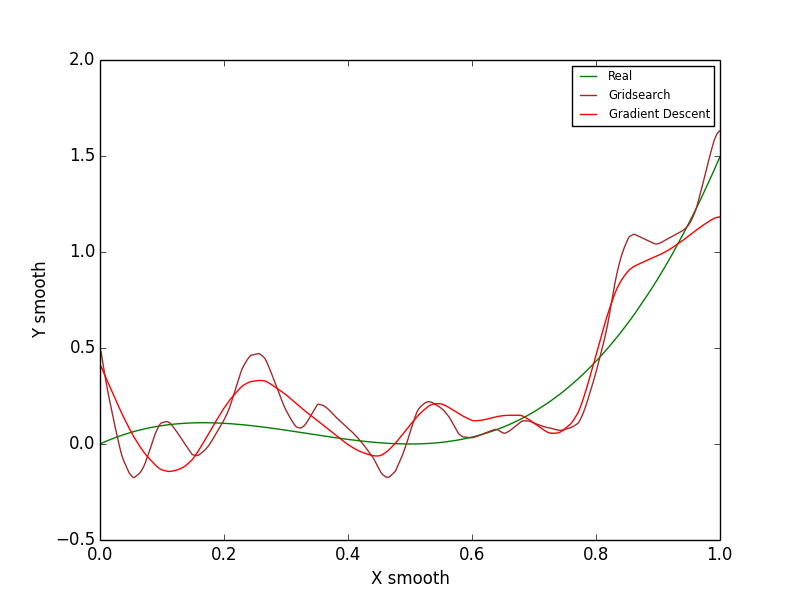
\includegraphics[height=40mm]{smooth_linear_thetas_2_100_20_6.png}
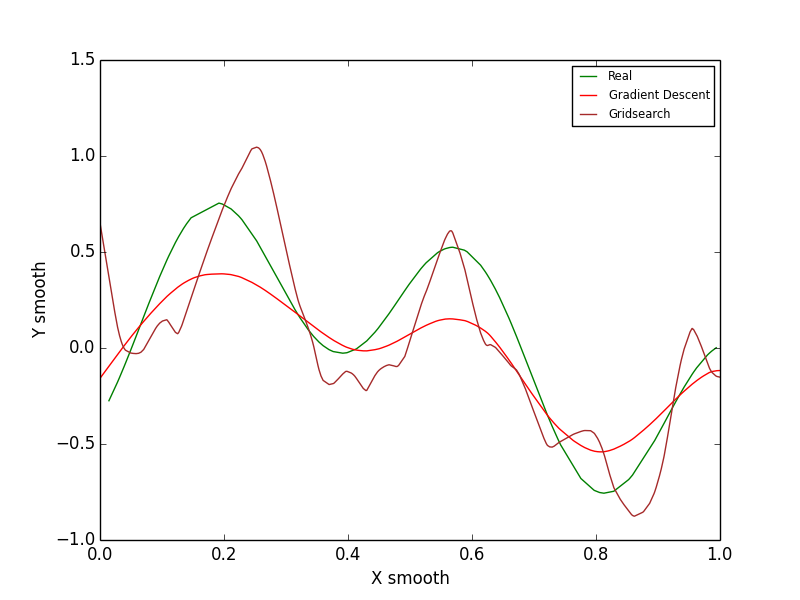
\includegraphics[height=40mm]{smooth_linear_thetas_0_100_20_6.png}
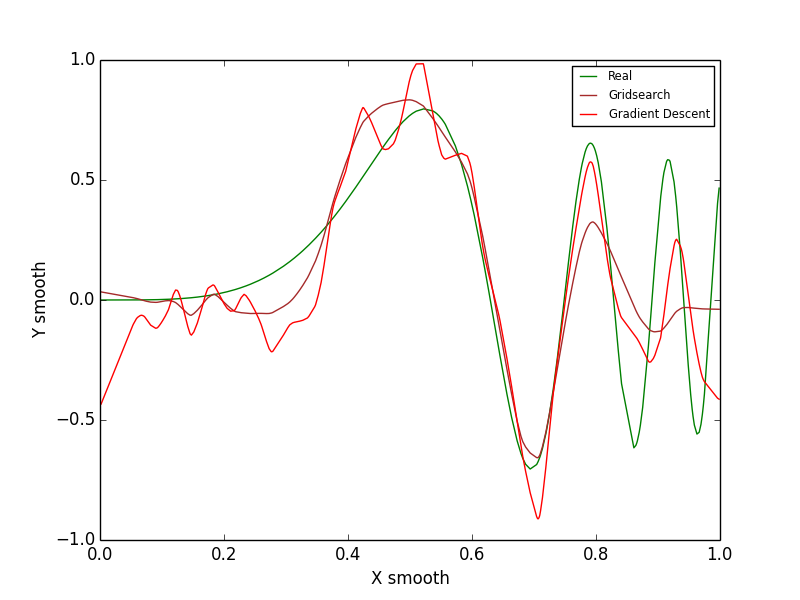
\includegraphics[height=40mm]{smooth_linear_thetas_1_100_20_6.png}
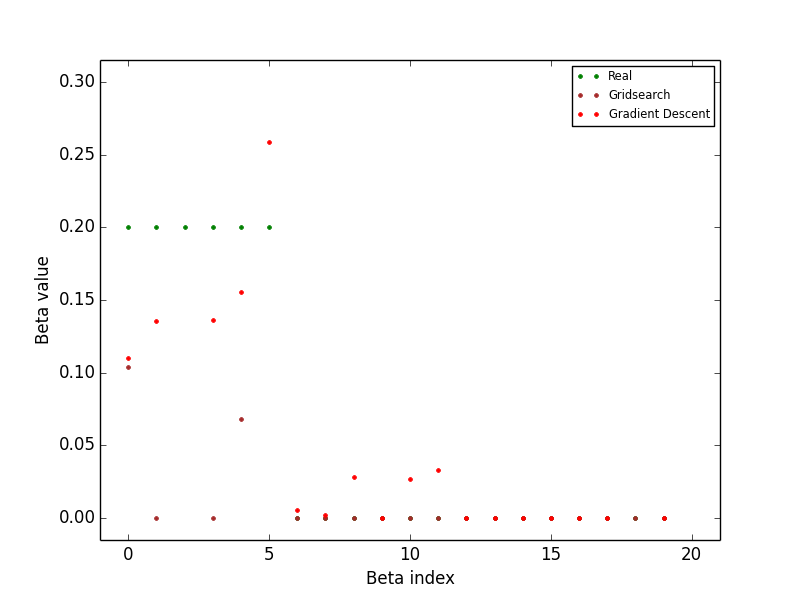
\includegraphics[height=40mm]{smooth_linear_beta_2_100_20_6.png}
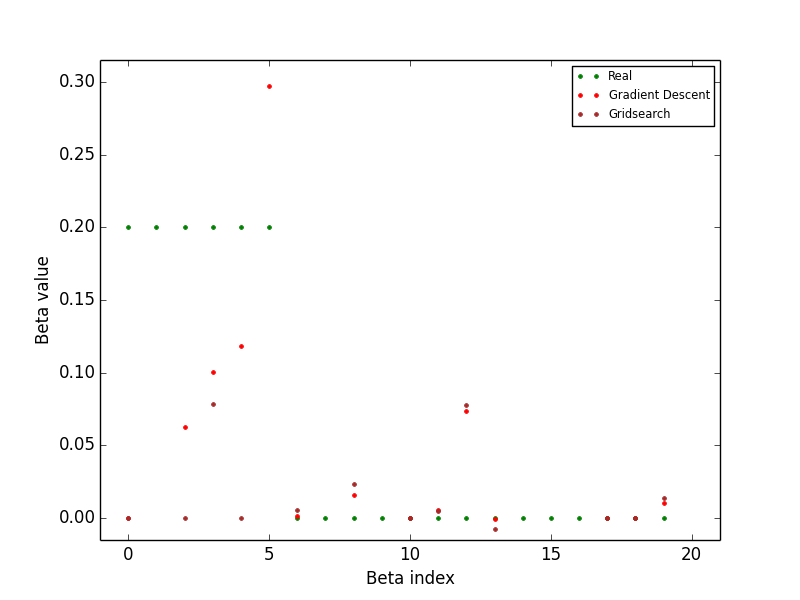
\includegraphics[height=40mm]{smooth_linear_beta_0_100_20_6.png}
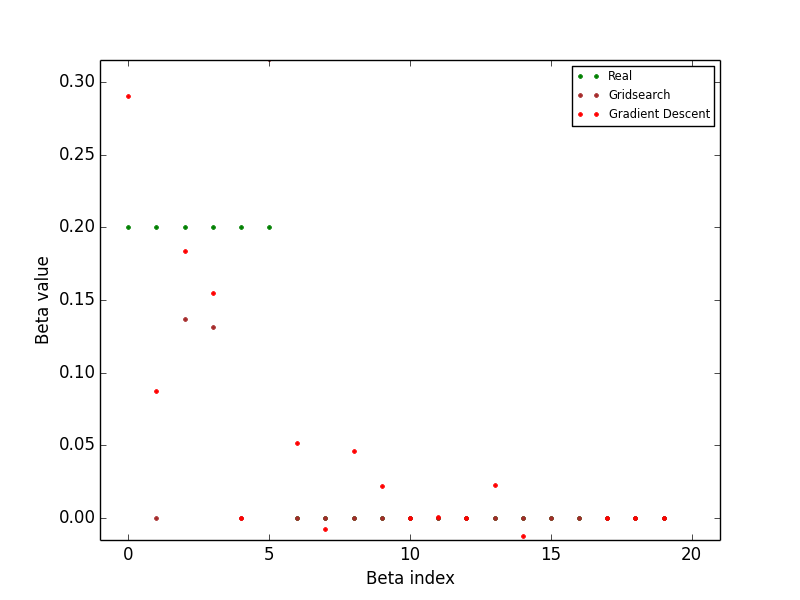
\includegraphics[height=40mm]{smooth_linear_beta_1_100_20_6.png}
\caption{Top: Example fits to the three smooth functions used in the experiments. The green line is the true function. Bottom: Example fits for the linear regression coefficients. The green is the true beta.}
\label{fig:modelfits}
\end{figure}

\section{Application to Real Data}
In this section, we discuss the performance and efficiency of joint optimization when applied to real data. We use un-pooled sparse group lasso as our example, since it can have the most number of penalty parameters among the regularization methods we previously mentioned. We compare this to sparse group lasso tuned using grid search.

We run regression to predict disease phenotype from gene expression data, as presented by Noah et. al. (2007). In this problem, the genes are grouped by gene pathways and we are interested in the pathways of interest and, from them, the driving genes.

Our dataset is from a colitis study of 127 total patients, 85 with colitis (59 crohn's patients + 26 ulcerative colitis patients) and 42 health controls (Burczynski 2006). Expression data was measured for 22,283 genes on affymetrix U133A microarrays. We grouped the genes according to the 326 C1 positional gene sets from MSigDb v5.0 (Subramanian 2005) and discarded the 2358 genes not found in the gene set. For each experiment, we randomly shuffled the data and used the first 50 observations for the training set and the remaining 77 for the test set. The experiment was repeated 10 times.

5-fold cross-validation was used to fit models. The penalty parameters in un-pooled sparse group lasso were all initialized at 0.5. For sparse group lasso, models were fit over a $5 \times 5$ grid of parameter values from 1e-4 to 5.

Perhaps the most important result is that joint optimization makes it possible to compare un-pooled sparse group lasso to sparse group lasso. Un-pooled sparse group lasso requires 327 regularization parameters for this problem, which is impossible to tune using grid search. Treating the problem as a continuous optimization problem not only makes it possible to tune many penalty parameters, but also makes the runtime comparable to grid search over two parameters, as seen in Table \ref{colitis}.

Un-pooled sparse group lasso and sparse group lasso achieve similar classification rates around 83\%. The primary difference is that un-pooled sparse group lasso finds solutions that are significantly more sparse than sparse group lasso -- on average, 9 genesets were identified, as opposed to 38. In addition, the number of genesets identified by un-pooled sparse group lasso has significantly lower variance. The number of genesets identified by sparse group lasso ranged from 2 to 73. The number of genesets identified by un-pooled sparse group lasso ranged from 8 to 12. Consistency is certainly an useful quality in regularization methods. These results suggest that un-pooling the penalty parameters in sparse group lasso can improve the regularization method. Further research is needed to determine if un-pooled sparse group lasso is a useful regularization method.

In this example, we have demonstrated that joint optimization is highly efficient at tuning parameters and can produce meaningful solutions to regression problems for real data.

\begin{table}
\begin{center}
\begin{tabular}{| l | l | l | l | l | }
\hline
 & \% correct  & Num. Genesets & Num. Genes & Runtime (sec) \\
\hline
SGL & 82.47 (0.7) & 38.4 (671.2) & 207.0 (22206.2) & 2722.4 \\
\hline
Unpooled SGL & 84.29 (0.3) & 8.9 (1.9) & 83.9 (664.5) & 2298.5 \\
\hline
\end{tabular}
\end{center}
\caption {Ulcerative Colitis Data: SGL = sparse group lasso, variance in parentheses}
\label{colitis}
\end{table}

\section{Discussion}
We proposed using joint optimization for tuning regularization parameters in both linear and nonlinear regressions. By treating the regression as an optimization problem over the regularization parameter space, joint optimization is highly scalable in the number of parameters. Through experiments on simulated data, we demonstrated that joint optimization is able to fit models with validation errors as low as grid search. We then increased the number of regularization parameters in traditional regularization methods and used joint optimization to fit even better models. During this exploration, we discovered that "unpooled" sparse group lasso has significantly better performance than the traditional sparse group lasso. Further research should be done to explore this new regularization method. Finally, we demonstrated that this method works well on real data.

This paper applied joint optimization to a number of criterions, but this method should be tested on more criterions to analyze its robustness. We also expect that by implementing joint optimization with more sophisticated optimization methods, we can expect significant gains in efficiency. Finally, it would be worthwhile to understand what types of situations are ill-suited for joint optimization and what is the maximum number of regularization parameters joint optimization can tune with reasonable computation time.

\section*{Appendix}

\subsection{Proof for Theorem \ref{thethrm}}

\begin{lemma}
Let the function $\hat f(\cdot)$ be defined as:
\begin{equation}
\hat f(\lambda) = \arg\min_f L(\beta, \lambda)
\end{equation}

For a given $\lambda_0$, let the $L(f, \lambda)$ be twice continuously differentiable with respect to $f$ in a neighborhood around $\hat f(\lambda_0)$ and that the hessian $Hess_f(L(f, \lambda_0))|_{\hat f(\lambda_0)}$ is nonsingular.
Then the objective function in the joint optimization problem is continuously differentiable in some neighborhood around $\lambda_0$.
\label{differentiablethrm}
\end{lemma}

\begin{proof}
Since the loss function and penalty functions are differentiable, the gradient at the optimal point $\hat\beta(\lambda_0)$ is zero:
\begin{equation}
\nabla_{\beta} L(\beta, \lambda) = 0
\end{equation}

Denote the expression on the left hand side as $H(f, \lambda_0)$. From our assumptions, we know that $H(f, \lambda_0)$ is continuously differentiable with respect to $f$ in some neighborhood of $\hat f(\lambda_0)$ and the Jacobian $D_\beta H(f, \lambda_0) |_{\hat f(\lambda_0)}$ is nonsingular. By the implicit function theorem, there exists a continuously differentiable function $\gamma$ such that 
\begin{equation}
H(\gamma(\lambda), \lambda) = 0
\end{equation}
and
$\hat f(\lambda) = \gamma(\lambda)$ within some neighborhood around $\lambda_0$.

\end{proof}

\begin{lemma}
Assume that the non-active set of $\hat f(\lambda_0)$ is locally constant in a neighborhood around a given $\lambda_0$ and that the assumptions in lemma \ref{differentiablethrm} hold for the active set of $\hat f(\lambda_0)$. Then within the neighborhood of $\lambda_0$, $\hat f(\lambda_0)$ is continuously differentiable in some neighborhood around $\lambda_0$.
\label{activesetthrm}
\end{lemma}

\begin{proof}
By the KKT conditions, the following subgradient condition is satisfied at the optimal point $\hat f(\lambda_0)$:

\begin{equation}
0 \in \partial_f L(f, \lambda_0)
\end{equation}

For the active set $\dot f(\lambda_0)$, the subgradient condition reduces to the gradient condition:

\begin{equation}
0 = \nabla_{\dot f} L(f, \lambda_0)
\label{gradientcondition}
\end{equation}

Applying Theorem \ref{differentiablethrm} to the gradient condition in (\ref{gradientcondition}), we know that the active set $\dot f(\cdot)$ is continuously differentiable in some neighborhood around $\lambda_0$. From our assumptions, the partial derivative of the non-active set of $\hat f$ is 0 for some neighborhood around $\lambda_0$. By combining the active and non-active sets, we have that $\hat f(\lambda_0)$ is continuously differentiable in some neighborhood around $\lambda_0$.

\end{proof}


\subsection{Elastic Net Gradient Derivations}
MATHS

\subsection{Sparse Group Lasso Derivations}

\subsubsection{Unpooled Sparse Group Lasso Derivations}
The gradient of the validation error with respect to the regularization parameters is:
\begin{equation}
\begin{array}{lcl}
\nabla_{\lambda_1^{(k)}} L(\boldsymbol y_V, X_V \hat \beta) &=& 
\frac{1}{n}
\Bigg (
X_V
(\frac{1}{n} X^T X + M_1 + M_2)^{-1}
\begin{bmatrix}
0 \\
\vdots \\
\frac{\hat\beta^{(l}}{||\hat\beta^{(l}||_2}\\
\vdots\\
0
\end{bmatrix}
\Bigg )^T
(\boldsymbol y_V - X_V \hat \beta)
 \\
\nabla_{\lambda_2} L(\boldsymbol y_V, X_V \hat \beta) &=&
\frac{1}{n}
\Bigg (
(\frac{1}{n} X^T X + M_1 + M_2)^{-1} sign(\hat \beta)
\Bigg )^T
(\boldsymbol y_V - X_V \hat \beta)
\\ 
\end{array}
\end{equation}

where $M_1$ is the block diagonal matrix with $l$ components 
$
\frac{\lambda_1^{(k)}}{|| \beta^{(k)}||_2^3}
\begin{bmatrix} 
\beta_1^{(k)} & 0 & \\
0 & \beta_2^{(k)} &  \\
 &  & \ddots \\
\end{bmatrix}
\begin{bmatrix}
\text{---} & \beta^{(k)T} & \text{---} \\
\text{---} & \beta^{(k)T} & \text{---} \\
\vdots
\end{bmatrix}
$ from top left to bottom right and $M_2$ is the diagonal matrix with $\frac{\lambda_1^{(k)}}{|| \beta^{(k)}||_2}$ from top left to bottom right.


\subsection{Additive Partial Linear Model Derivations}

\subsubsection{Additive Partial Linear Model Derivations: 3-penalties}

To perform joint optimization, we formulate the problem as follows:
\begin{multline}
\min_{\lambda_1, \lambda_2, \lambda_3} \frac{1}{2} \bigl\lvert\bigl\lvert \boldsymbol y_V - X_V\hat\beta - M_V \hat\theta \bigl\rvert\bigl\rvert^2_2 \\
\text{ where } \hat\beta, \hat\theta = \arg\min_{\beta, \theta} \frac{1}{2} \bigl\lvert\bigl\lvert y - X\beta - M_T \theta \bigl\rvert\bigl\rvert^2_2
+ \lambda_1 \lvert\lvert \beta \rvert \rvert_1
+ \frac{1}{2} \lambda_2 \lvert\lvert \beta \rvert \rvert_2^2
+ \frac{1}{2} \lambda_3 \lvert\lvert D^{(2)} \theta \rvert \rvert_2^2
\end{multline}
where $M_V \in \mathbb{R}^{|V| \times n}$ is the matrix such that $M_V X = X_V$ and $M_T \in \mathbb{R}^{|T| \times n}$ is the matrix such that $M_T X = X_T$ .

The gradients of the validation set error with respect to the regularization parameters are:
\begin{equation}
\nabla_{\lambda_i} L(\boldsymbol y_V, X_V \hat \beta + \hat \theta) = (X_V \frac{\partial \beta}{\partial \lambda_i} + M_V \frac{\partial \theta}{\partial \lambda_i})^T(\boldsymbol y_V - X_V \hat \beta - \hat \theta_V)
\end{equation}
where
\begin{equation}
\begin{array}{lcl}
\frac{\partial \beta}{\partial \lambda_1} &=& -(X_T^T X_T - X_T^T M_T(M_T^T M_T + \lambda_3 D^TD)^{-1} M_T^T X_T + \lambda_2 I)^{-1} sign(\hat \beta) \\
\frac{\partial \theta}{\partial \lambda_1} &=& -(M_T^T M_T + \lambda_3 D^T D)^{-1}  M_T^T X_T \frac{\partial \beta}{\partial \lambda_1}
\\
\frac{\partial \beta}{\partial \lambda_2} &=& -(X_T^T X_T - X_T^T M_T(M_T^T M_T + \lambda_3 D^TD)^{-1} M_T^T X_T + \lambda_2 I)^{-1} \hat \beta \\
\frac{\partial \theta}{\partial \lambda_2} &=& -(M_T^T M_T + \lambda_3 D^T D)^{-1}  M_T^T X_T \frac{\partial \beta}{\partial \lambda_2}
\\
\frac{\partial \theta}{\partial \lambda_3} &=& -(M_T^T M_T - M_T^T X_T (X_T^TX_T + \lambda_2 I)^{-1} X_T^T M_T + \lambda_3 D^TD)^{-1} D^TD \theta
\\
\frac{\partial \beta}{\partial \lambda_3} &=& - (X_T^TX_T + \lambda_2 I)^{-1} X_T^T M_T \frac{\partial \theta}{\partial \lambda_3} \\
\end{array}
\end{equation}

\section*{Acknowledgments}
BLAH


%\section*{References}
% Either type in your references using
% \begin{thebibliography}{}
% \bibitem{}
% Text
% \end{thebibliography}
%
% OR
%
% Compile your BiBTeX database using our plos2009.bst
% style file and paste the contents of your .bbl file
% here.
% 
\begin{thebibliography}{10}
\bibitem{bib1}
Lorem M, Ipsum VE (1990) Rank Correlation Methods. New York: Oxford University Press, 5th edition.

\end{thebibliography}

\end{document}

